\section{Materials}\label{sec:materials}

\subsection{Data}\label{sec:data}

The multi-parametric \ac{mri} data are acquired from a cohort of patients with higher-than-normal level of \ac{psa}.
The acquisition is performed using a 3T whole body \ac{mri} scanner (Siemens Magnetom Trio TIM, Erlangen, Germany) using sequences to obtain \ac{t2w}-\ac{mri}, \ac{dce}-\ac{mri} and \ac{dw}-\ac{mri}.
Aside of the \ac{mri} examination, these patients also have underwent a guided-biopsy.
The dataset is composed of a total of 20 patients of which 18 patients have biopsy proven \ac{cap} and 2 patients are ``healthy'' with negative biopsies.
Therefore, 13 patients have a \ac{cap} in the \ac{pz}, 3 patients have \ac{cap} in the \ac{cg}, 2 patients have invasive \ac{cap} in both \ac{pz} and \ac{cg} and finally 2 patients are considered as ``healthy''.
An experienced radiologist has segmented the prostate organ --- on \ac{t2w}-\ac{mri} and \ac{dce}-\ac{mri} --- as well as the prostate zones (i.e., \ac{pz} and \ac{cg}) and \ac{cap} on the \ac{t2w}-\ac{mri}.

A \SI{3}{\mm} slice fat-suppressed \ac{t2w} fast spin-echo sequence (\ac{tr}/\ac{te}/\ac{etl}: \SI{3400}{\ms}/\SI{85}{\ms}/13) is used to acquire images in sagittal and oblique coronal planes, the latter planes being orientated perpendicular or parallel to the prostate \ac{pz} – rectal wall axis.
Three-dimensional \ac{t2w} fast spin-echo (\ac{tr}/\ac{te}/\ac{etl}: \SI{3600}{\ms}/\SI{143}{\ms}/109, slice thickness: \SI{1.25}{\mm}) images are then acquired in an oblique axial plane.
The nominal matrix and \ac{fov} of the 3D \ac{t2w} fast spin-echo images are $320 \times 256$ and $280 \times 240$ mm\textsuperscript{2}, respectively, thereby affording sub-millimetric pixel resolution within the imaging plane.

\ac{dce}-\ac{mri} are performed using a fat suppressed 3D T$_1$ VIBE sequence (\ac{tr}/\ac{te}/Flip angle: \SI{3.25}{\ms}/\SI{1.12}{\ms}/\SI{10}{\degree}; Matrix: $256 \times 192$; \ac{fov}: $280 \times 210$ (with 75\% rectangular \ac{fov}); slab of 16 partitions of \SI{3.5}{\mm} thickness; temporal resolution: \SI{6}{\s}/slab over approximately \SI{5}{\minute}).
A power injector (Medrad, Indianola, USA) is used to provide a bolus injection of Gd-DTPA (Dotarem, Guerbet, Roissy, France) at a dose of \SI{0.2}{\ml} Gd-DTPA/kg of body weight.

These \ac{dce}-\ac{mri} sequences are resampled using the spatial information of the \ac{t2w}-\ac{mri} and missing data are interpolated using linear interpolation.
The volumes of the \ac{dce}-\ac{mri} dynamic are rigidly registered, to remove any patient motion during the acquisition.
Furthermore, a non-rigid registration is performed between the \ac{t2w}-\ac{mri} and \ac{dce}-\ac{mri} in order to propagate the prostate zones and \ac{cap} ground-truths.
The resampling is implemented in C++ using the Insight Segmentation and Registration Toolkit~\citep{ibanez2005itk}.

\subsection{Implementation}

The implementation of the registration (C++), normalization (Python), and classification pipeline (Python) are publicly available on GitHub\footnote{\url{https://github.com/I2Cvb/lemaitre-2016-nov/tree/master}}.
The data used for this work are also publicly available\footnote{\url{http://kaggle.com}}.

\section{Experiments and results}\label{sec:experiments}

\subsection{Classification of individual parameter for each model}

% \begin{table}
%   \caption{\acs*{auc} of the individual features for each method.}
%   \centering
%   \begin{tabular}{l c c c c}
%     \toprule
%     \textbf{Features} & \multicolumn{2}{c}{Un-normalized data} & \multicolumn{2}{c}{Normalized data} \\
%     & \acs*{rf} & \acs*{nb} & \acs*{rf} & \acs*{nb} \\
%     \midrule
%     \textbf{Brix model} & & & & \\
%     \quad $A$         & 0.54 & 0.62 & 0.58 & 0.67 \\
%     \quad $k_{el}$    & 0.55 & 0.52 & 0.54 & 0.61 \\
%     \quad $k_{ep}$    & 0.51 & 0.52 & 0.51 & 0.58 \\
%     \textbf{Hoffmann model} & & & & \\
%     \quad $A$         & 0.52 & 0.50 & 0.51 & 0.56 \\
%     \quad $k_{el}$    & 0.55 & 0.53 & 0.54 & 0.64 \\
%     \quad $k_{ep}$    & 0.55 & 0.50 & 0.53 & 0.66 \\
%     \textbf{Tofts model with population \ac{aif}} & & & & \\
%     \quad $K_{trans}$ & 0.56 & 0.62 & 0.56 & 0.65 \\
%     \quad $v_{e}$     & 0.51 & 0.50 & 0.50 & 0.52 \\
%     \quad $v_{p}$     & 0.53 & 0.63 & 0.55 & 0.53 \\
%     \textbf{Tofts model with patient \ac{aif}} & & & & \\
%     \quad $K_{trans}$ & 0.57 & 0.66 & 0.56 & 0.65 \\
%     \quad $v_{e}$     & 0.49 & 0.50 & 0.51 & 0.52 \\
%     \quad $v_{p}$     & 0.53 & 0.37 & 0.57 & 0.65 \\
%     \textbf{\ac{pun} model} & & & & \\
%     \quad $a_0$       & 0.52 & 0.53 & 0.53 & 0.51  \\
%     \quad $r$         & 0.53 & 0.59 & 0.55 & 0.55 \\
%     \quad $\beta$     & 0.55 & 0.56 & 0.53 & 0.44 \\
%     \textbf{Semi-quantitative analysis} & & & & \\
%     \quad wash-in     & 0.59 & 0.64 & 0.55 & 0.51 \\
%     \quad wash-out    & 0.52 & 0.50 & 0.56 & 0.66 \\
%     \quad IAUC        & 0.51 & 0.61 & 0.52 & 0.64 \\
%     \quad $\tau$      & 0.57 & 0.57 & 0.56 & 0.61 \\
%     \quad $S_M - S_0$ & 0.56 & 0.63 & 0.53 & 0.64 \\
%     \bottomrule
%   \end{tabular}
%   \label{tab:resfeats}
% \end{table}

The first experiment consists in comparing the classification performance using each individual parameter for the different models, to assess the potential benefit of the normalization method.
Therefore, each feature is individually classified using a Gaussian \ac{nb} classifier in a \ac{lopo} fashion.
{\color{red}\ac{nb} is used due to its simplicity and it enables to check the fitted parameters for interpretation.}
The results are summarized in Table~\ref{tab:resfeats}.
It can be noted that in the majority of the cases, normalizing the data improve the classification performance in terms of \ac{auc}.
Only the \ac{pun} model does not follow this tendency {\color{red} which might due to the fact that the function do not fit the data as good as the other model - WE WILL NEED SOME RMSE FOR EACH FITTING IF WE SAY SO.}.

{\color{red}It could be interesting to check the value of the mean and std of the \ac{nb}. We could compute a ratio which refer to the class separability.}

\begin{table}
  \caption{\acs*{auc} for each individual pharmacokinetic parameter using a \acs*{nb} classifier.}
  \centering
  \begin{tabular}{l c c}
    \toprule
    \textbf{Features} & Un-normalized data & Normalized data \\
    \midrule
    \textbf{Brix model} & & \\
    \quad $A$         & 0.62 & 0.67 \\
    \quad $k_{el}$    & 0.52 & 0.61 \\
    \quad $k_{ep}$    & 0.52 & 0.58 \\
    \textbf{Hoffmann model} & & \\
    \quad $A$         & 0.50 & 0.56 \\
    \quad $k_{el}$    & 0.53 & 0.64 \\
    \quad $k_{ep}$    & 0.50 & 0.66 \\
    \textbf{Tofts model with population \ac{aif}} & & \\
    \quad $K_{trans}$ & 0.62 & 0.65 \\
    \quad $v_{e}$     & 0.50 & 0.52 \\
    \quad $v_{p}$     & 0.63 & 0.53 \\
    \textbf{Tofts model with patient \ac{aif}} & & \\
    \quad $K_{trans}$ & 0.66 & 0.65 \\
    \quad $v_{e}$     & 0.50 & 0.52 \\
    \quad $v_{p}$     & 0.37 & 0.65 \\
    \textbf{\ac{pun} model} & & \\
    \quad $a_0$       & 0.53 & 0.51 \\
    \quad $r$         & 0.59 & 0.55 \\
    \quad $\beta$     & 0.56 & 0.44 \\
    \textbf{Semi-quantitative analysis} & & \\
    \quad wash-in     & 0.64 & 0.51 \\
    \quad wash-out    & 0.50 & 0.66 \\
    \quad IAUC        & 0.61 & 0.64 \\
    \quad $\tau$      & 0.57 & 0.61 \\
    \quad $S_M - S_0$ & 0.63 & 0.64 \\
    \bottomrule
  \end{tabular}
  \label{tab:resfeats}
\end{table}

\subsection{Classification by combining the parameters for each model}

Usually, the parameters are combined to form a multi-dimensional prior to classify the data.
Therefore, for each model, all parameters are combined and classified using a \ac{rf} classifier in a \ac{lopo} fashion.
The use of \ac{rf} is motivated since that it leads to the best performance in the state-of-the-art methods~\citep{litjens2014computer}.
The results are summarized by making \ac{roc} analysis and computing the \ac{auc}, as reported in Fig.\,\ref{fig:normpharmarf}.
It can be noted that in all the cases the normalization of the data improve the classification performance.

\begin{figure}
  \centering
  \hspace*{\fill}
  \subfigure[Without normalization.]{\label{fig:rfpharmaunorm}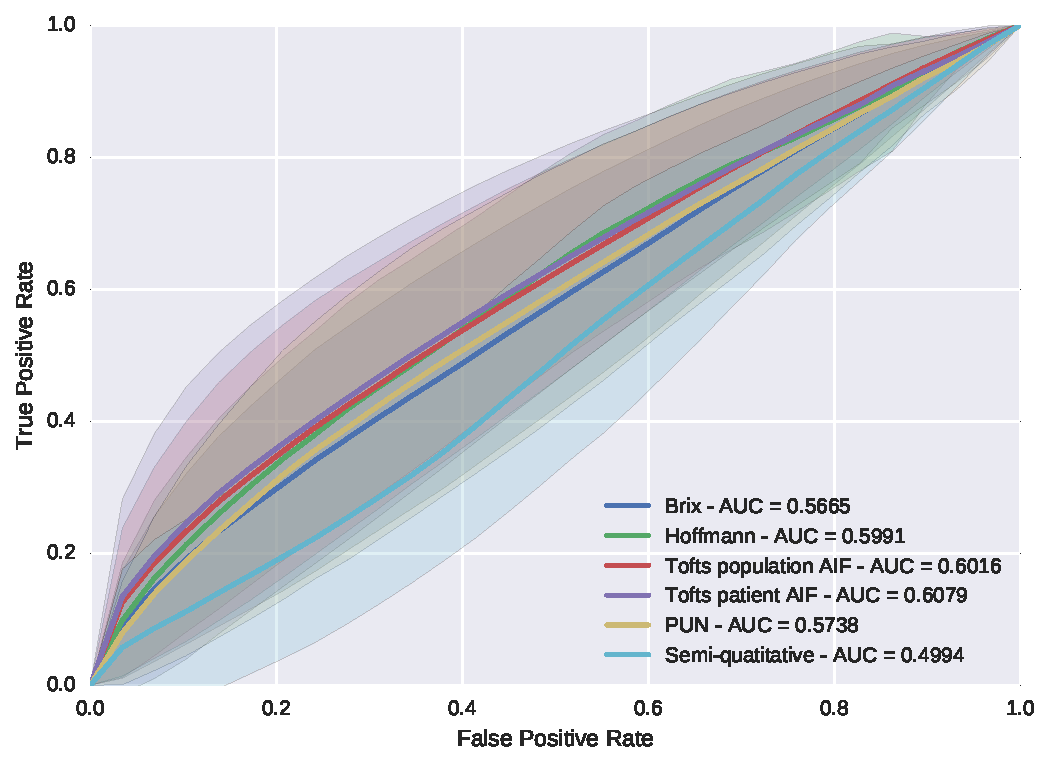
\includegraphics[width=.49\textwidth]{03_experiments/figures/unormalized/rf.pdf}} \hfill
  \subfigure[With normalization.]{\label{fig:rfpharmanorm}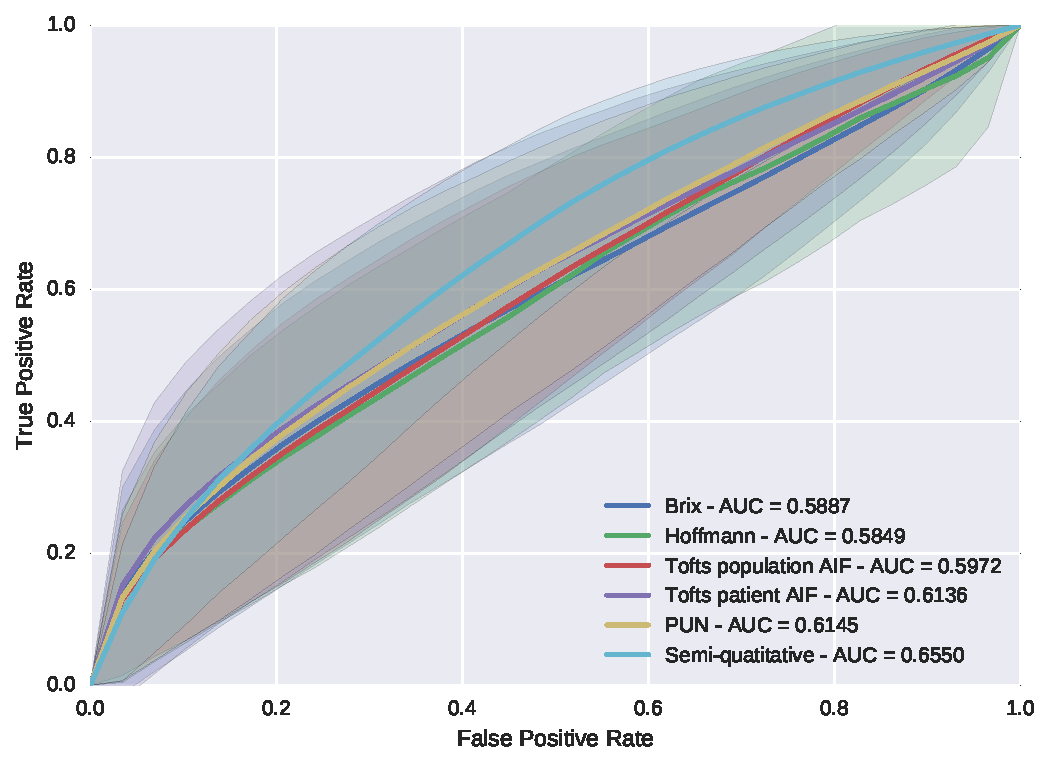
\includegraphics[width=.49\textwidth]{03_experiments/figures/normalized/rf.pdf}}
  \hspace*{\fill}
  \caption{\acs*{roc} analysis using a \acs*{rf} classifier with and without normalization \ac{dce}-\ac{mri} data for different pharmacokinetic models.}
  \label{fig:normpharmarf}
\end{figure}

% \begin{figure}
%   \centering
%   \hspace*{\fill}
%   \subfigure[Without normalization.]{\label{fig:nbpharmaunorm}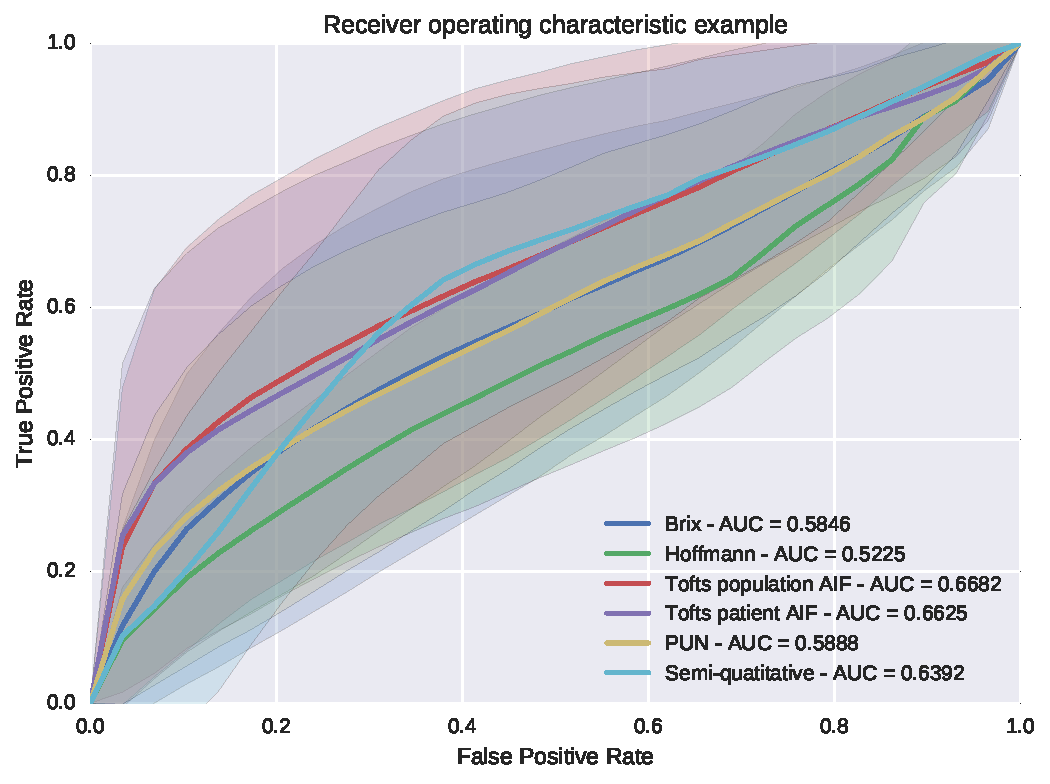
\includegraphics[width=.49\textwidth]{03_experiments/figures/unormalized/nb.pdf}} \hfill
%   \subfigure[With normalization.]{\label{fig:nbpharmanorm}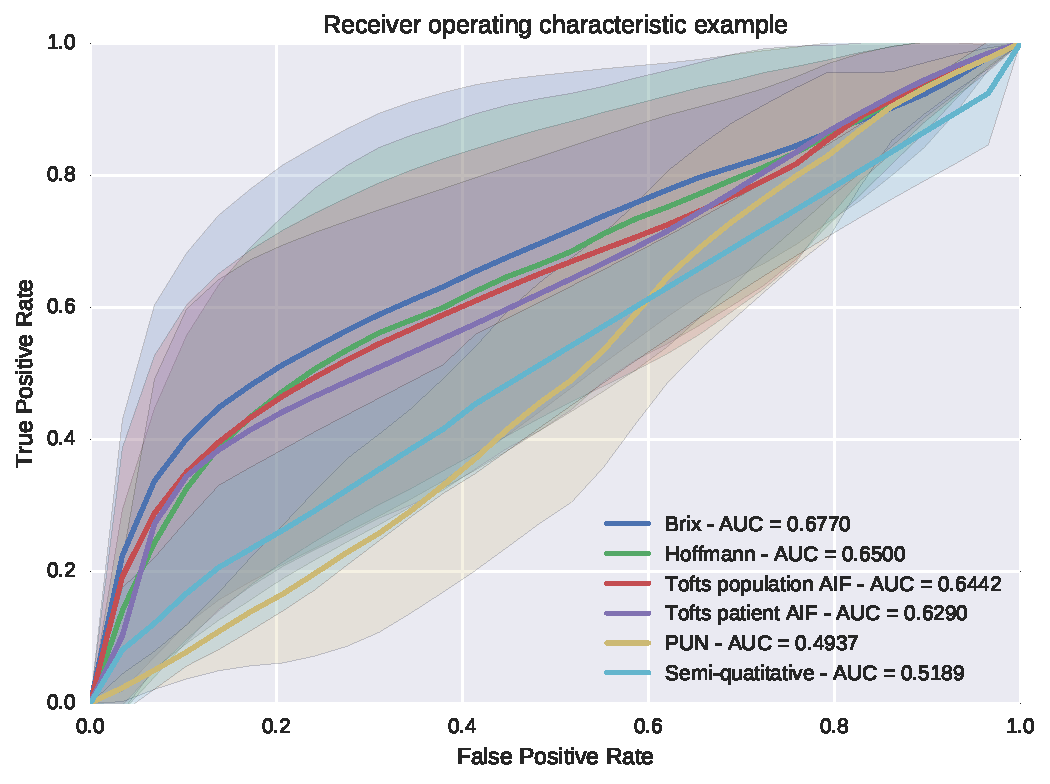
\includegraphics[width=.49\textwidth]{03_experiments/figures/normalized/nb.pdf}}
%   \hspace*{\fill}
%   \caption{\acs*{roc} analysis using a \acs*{nb} classifier with and without normalization \ac{dce}-\ac{mri} data for different pharmacokinetic models.}
%   \label{fig:normpharmanb}
% \end{figure}

% \begin{figure}
%   \centering
%   \hspace*{\fill}
%   \subfigure[\acs*{rf} classifier.]{\label{fig:rfunorm}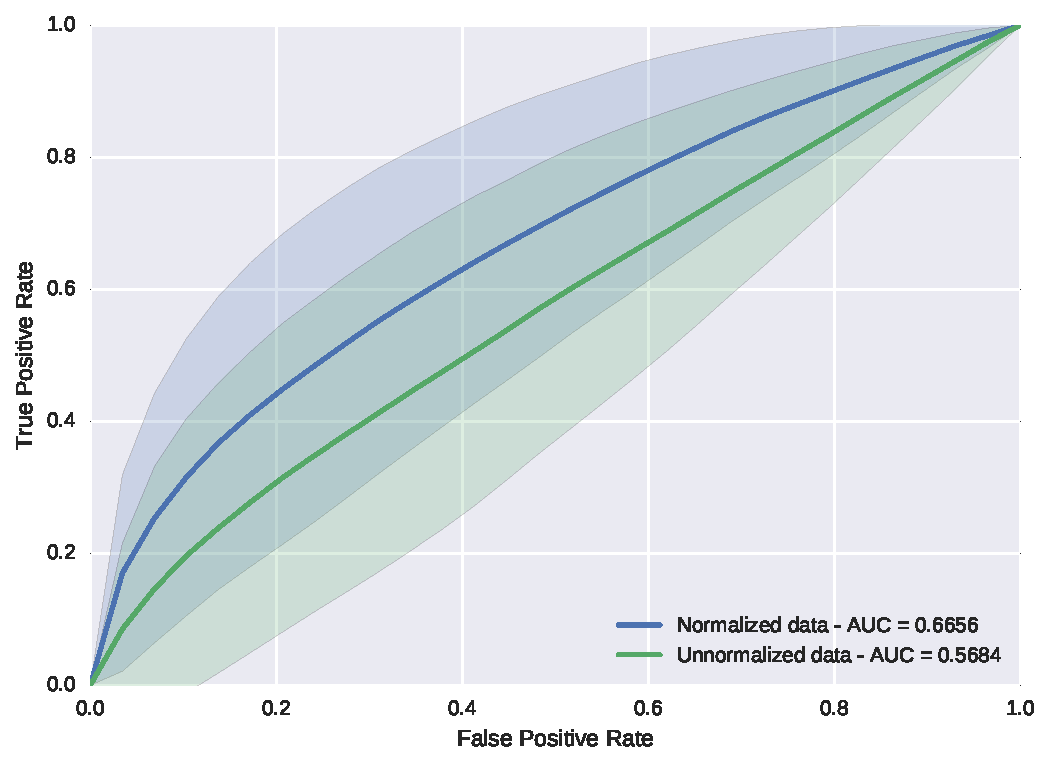
\includegraphics[width=.49\textwidth]{03_experiments/figures/rf.pdf}} \hfill
%   \subfigure[\acs*{nb} classifier.]{\label{fig:nbunorm}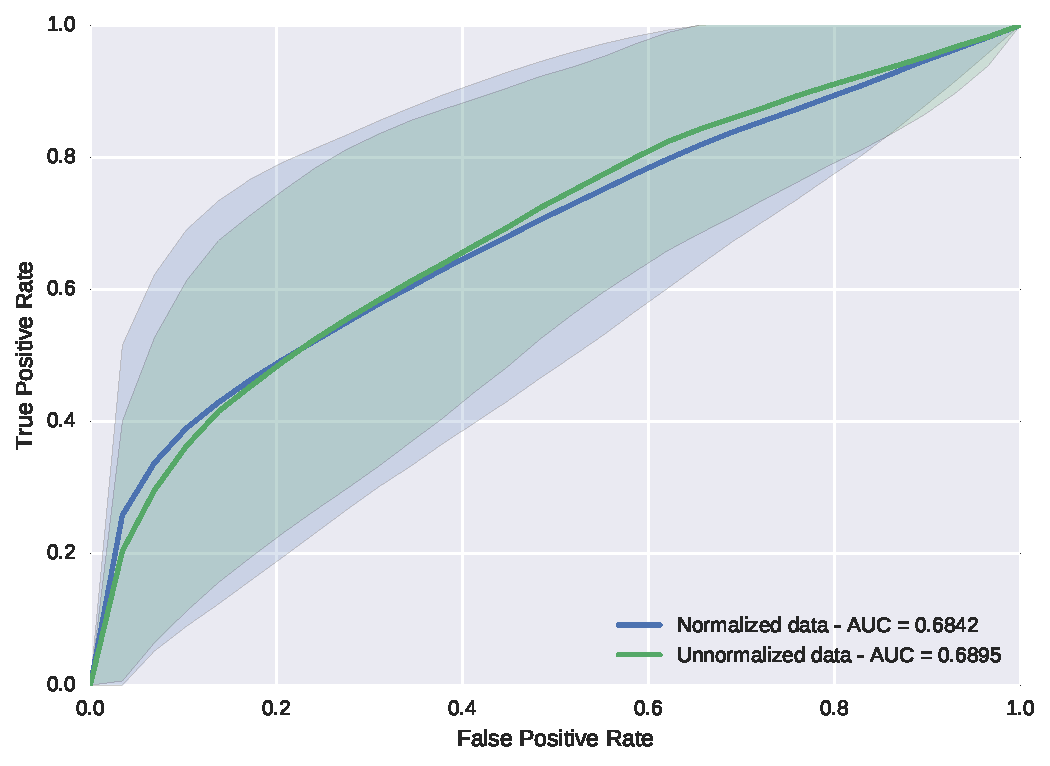
\includegraphics[width=.49\textwidth]{03_experiments/figures/nb.pdf}}
%   \hspace*{\fill}
%   \caption{\acs*{roc} analysis using the entire \ac{dce}-\ac{mri} signal with and without normalization.}
%   \label{fig:unormdcesignal}
% \end{figure}

\subsection{Classification of the entire enhanced \acs*{dce}-\acs*{mri} signal}

The quantification methods are extracting a minimal set of parameters which should characterized the enhancement \ac{dce}-\ac{mri} curves.
However, this extraction could discard some information of the signal.
This experiment attends to use the whole \ac{dce}-\ac{mri} signal to perform the classification.
Therefore, the enhanced signal is classified using a \ac{rf} classifier in a \ac{lopo} fashion.
The \ac{roc} analysis and \ac{auc} are reported in Fig.\,\ref{fig:rfnormdcesignal}.
It can be note that the worst performance are achieved while data without normalization.
However, normalizing the data, this classification strategy lead the best classification performance, outperforming any quantification method, showing the importance of our normalization algorithm.

\begin{figure}
  \centering
  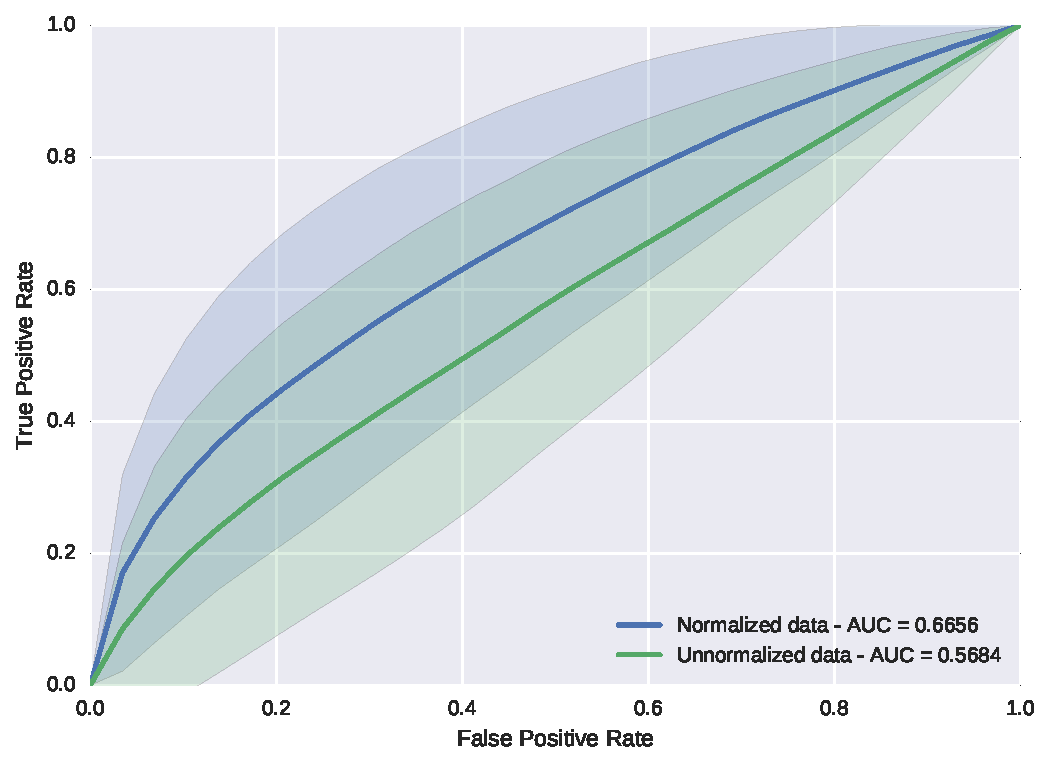
\includegraphics[width=0.7\linewidth]{03_experiments/figures/rf.pdf}
  \caption{\acs*{roc} analysis using the entire \ac{dce}-\ac{mri} signal with and without normalization in conjunction with a \acs*{rf} classifier.}
  \label{fig:rfnormdcesignal}
\end{figure}

%%% Local Variables: 
%%% mode: latex
%%% TeX-master: "../main"
%%% End: 
